\section{多元Laplace分布}
\label{sec:mvd-laplace}

t分布的重尾有代价：自由度小的时候，方差甚至均值都不存在。有些波动比高斯更“尖”、尾部更厚，却仍有全部有限阶矩，一元时第~\ref{chap:common-distributions}章的Laplace分布正适合描述它们。它的密度是$(2b)^{-1}\mathrm{e}^{-\lvert x-\mu\rvert/b}$，尾部按指数衰减，比高斯的$\mathrm{e}^{-x^{2}/2}$慢，但仍快过任何负幂。

推广到多元，答案并不唯一。最直接的做法是让各分量独立地服从一元Laplace分布；另一种做法沿用上一节的思路，用一个共同的随机尺度放大高斯向量。本节采用后者，即由共同指数尺度混合得到的对称椭圆型版本，称为\term{多元Laplace分布}（multivariate Laplace distribution），并在最后与独立分量的乘积模型对照。

\subsection{正态指数混合}
\label{sec:mvd-laplace-mixture}

\paragraph{构造}
上一节的共同尺度$\nu/U$有很长的右尾，这是t分布矩不存在的根源。换一个右尾短的尺度，就能保留混合带来的厚尾，又不丢掉矩。指数分布是最简单的选择。

\begin{definition}[多元Laplace分布]
\label{def:mvd-laplace}
设$\bm{\mu}\in\mathbb{R}^{d}$，$\bm{\Sigma}$是$d\times d$正定矩阵。$W\sim\operatorname{Exp}(1)$（速率为$1$）与$\bm{Z}\sim\mathcal{N}(\bm{0},\bm{\Sigma})$相互独立，令
\begin{equation}
 \bm{X}=\bm{\mu}+\sqrt{W}\,\bm{Z} .
 \label{eq:mvd-laplace-construction}
\end{equation}
称$\bm{X}$服从参数为$\bm{\mu}$、$\bm{\Sigma}$的多元Laplace分布。
\end{definition}

固定$W=w$，$\bm{X}\sim\mathcal{N}(\bm{\mu},w\bm{\Sigma})$，所以这仍是一个正态尺度混合，只是这次混合的是方差因子$W$本身。图~\ref{fig:mvd-mixing-laws}比较两种方差因子：$\nu=5$的t分布用$5/U$，本节用$W$。两者都可以取远大于$1$的值，这是厚尾的来源；但$W$的尾概率是$\mathrm{e}^{-v}$，$5/U$的尾概率只按$v^{-5/2}$下降。

\begin{BookInlineFigure}
  \centering
  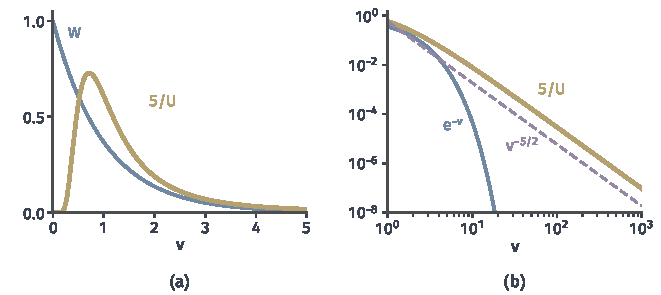
\includegraphics[width=112mm]{figures/07-probability/01-elementary-probability/matplotlib/mvd-mixing-laws/figure.pdf}
  \caption{两种正态尺度混合的方差因子。(a)密度：多元Laplace的$W\sim\operatorname{Exp}(1)$（蓝）与$\nu=5$的多元t的$5/U$，$U\sim\chi^2_5$（黄）。(b)尾概率$\mathbb{P}(\cdot>v)$，双对数坐标；紫色虚线是斜率为$-5/2$的参考线。尾概率由精确密度数值积分得到。}
  \label{fig:mvd-mixing-laws}
\end{BookInlineFigure}

\paragraph{均值、协方差与矩}
$\sqrt W$的均值$\Gamma(3/2)=\sqrt\pi/2$有限，由独立性及$\mathbb{E}[\bm{Z}]=\bm{0}$，$\mathbb{E}[\bm{X}]=\bm{\mu}$。协方差为
\begin{equation}
 \operatorname{Cov}(\bm{X})=\mathbb{E}[W]\,\bm{\Sigma}=\bm{\Sigma} .
 \label{eq:mvd-laplace-cov}
\end{equation}
与t分布不同，这里的$\bm{\Sigma}$就是协方差矩阵。

更高阶的矩同样存在。对任意$k\geq0$，$\mathbb{E}[W^{k/2}]=\Gamma(1+k/2)<\infty$，而高斯分量的各阶矩都有限，所以
\[
 \mathbb{E}\lvert X_i-\mu_i\rvert^{k}=\Gamma\Bigl(1+\frac k2\Bigr)\,\mathbb{E}\lvert Z_i\rvert^{k}<\infty .
\]
这正是选用指数尺度的目的：混合让尾部变厚，指数尺度的短尾又保证一切矩有限。

\paragraph{联合密度}
由式~\eqref{eq:mvd-scale-mixture-density}，把$g_u$换成$\mathcal{N}(\bm{\mu},w\bm{\Sigma})$的密度、$f_U$换成$\mathrm{e}^{-w}$，
\begin{equation}
 f_{\bm{X}}(\bm{x})=\frac{1}{(2\pi)^{d/2}(\det\bm{\Sigma})^{1/2}}\int_0^{\infty}w^{-d/2}\exp\Bigl(-w-\frac{Q(\bm{x})}{2w}\Bigr)\,\mathrm{d}w .
 \label{eq:mvd-laplace-density}
\end{equation}
密度仍只通过$Q(\bm{x})$依赖$\bm{x}$，所以多元Laplace分布也是椭圆分布，等密度面与$\mathcal{N}(\bm{\mu},\bm{\Sigma})$的相同。剩下的问题是沿着椭球向外，密度怎样衰减。下面的积分让我们在$d=1$和$d=3$时算出初等形式。

\begin{lemma}[一个指数积分]
\label{lem:mvd-exp-integral}
对$a>0$，
\begin{equation}
 \begin{aligned}
  \int_0^{\infty}w^{-1/2}\mathrm{e}^{-w-a/w}\,\mathrm{d}w&=\sqrt\pi\,\mathrm{e}^{-2\sqrt a},\\
  \int_0^{\infty}w^{-3/2}\mathrm{e}^{-w-a/w}\,\mathrm{d}w&=\sqrt{\frac{\pi}{a}}\,\mathrm{e}^{-2\sqrt a} .
 \end{aligned}
 \label{eq:mvd-exp-integral}
\end{equation}
\end{lemma}

\begin{proof}
第一个积分中令$w=s^{2}$，$\mathrm{d}w=2s\,\mathrm{d}s$，再记$c=\sqrt a$并在指数中配方，$s^{2}+c^{2}/s^{2}=(s-c/s)^{2}+2c$，于是
\[
 \int_0^{\infty}w^{-1/2}\mathrm{e}^{-w-a/w}\,\mathrm{d}w=2\int_0^{\infty}\mathrm{e}^{-s^{2}-c^{2}/s^{2}}\,\mathrm{d}s=2\mathrm{e}^{-2c}J,
\]
其中
\[
 J=\int_0^{\infty}\mathrm{e}^{-(s-c/s)^{2}}\,\mathrm{d}s .
\]

求$J$用一个对称技巧。令$s=c/t$，$\mathrm{d}s=-c\,t^{-2}\mathrm{d}t$，积分限对调，$(s-c/s)^{2}=(c/t-t)^{2}$，所以
\[
 J=\int_0^{\infty}\mathrm{e}^{-(t-c/t)^{2}}\,\frac{c}{t^{2}}\,\mathrm{d}t .
\]
把两种写法相加，
\[
 2J=\int_0^{\infty}\mathrm{e}^{-(s-c/s)^{2}}\Bigl(1+\frac{c}{s^{2}}\Bigr)\,\mathrm{d}s .
\]
再令$y=s-c/s$，它在$(0,\infty)$上严格递增，从$-\infty$变到$\infty$，且$\mathrm{d}y=(1+c/s^{2})\,\mathrm{d}s$，
\[
 2J=\int_{-\infty}^{\infty}\mathrm{e}^{-y^{2}}\,\mathrm{d}y=\sqrt\pi .
\]
所以$J=\sqrt\pi/2$，第一个等式成立。

第二个积分由第一个换元得到。在第一个积分中令$w=a/t$，$\mathrm{d}w=-a\,t^{-2}\mathrm{d}t$，$w^{-1/2}=t^{1/2}a^{-1/2}$，指数$-w-a/w$变为$-a/t-t$，于是
\[
 \sqrt\pi\,\mathrm{e}^{-2\sqrt a}=\int_0^{\infty}t^{1/2}a^{-1/2}\,\mathrm{e}^{-t-a/t}\,\frac{a}{t^{2}}\,\mathrm{d}t=\sqrt a\int_0^{\infty}t^{-3/2}\mathrm{e}^{-t-a/t}\,\mathrm{d}t .
\]
两边除以$\sqrt a$即得第二个等式。
\end{proof}

$d=1$时$\bm{\Sigma}=\sigma^{2}$，$Q=(x-\mu)^{2}/\sigma^{2}$。式~\eqref{eq:mvd-laplace-density}中取$a=Q/2$，用式~\eqref{eq:mvd-exp-integral}的第一式，$2\sqrt a=\sqrt2\,\lvert x-\mu\rvert/\sigma$，
\[
 f_X(x)=\frac{1}{\sqrt{2\pi}\,\sigma}\sqrt\pi\,\mathrm{e}^{-\sqrt2\lvert x-\mu\rvert/\sigma}=\frac{1}{\sqrt2\,\sigma}\mathrm{e}^{-\sqrt2\lvert x-\mu\rvert/\sigma} .
\]
这正是尺度$b=\sigma/\sqrt2$的一元Laplace密度，其方差$2b^{2}=\sigma^{2}$与式~\eqref{eq:mvd-laplace-cov}一致。

$d=3$时用第二式，同样取$a=Q/2$，常数$(2\pi)^{-3/2}\sqrt{2\pi}=(2\pi)^{-1}$，得到
\[
 f_{\bm{X}}(\bm{x})=\frac{1}{2\pi(\det\bm{\Sigma})^{1/2}}\cdot\frac{\mathrm{e}^{-\sqrt{2Q(\bm{x})}}}{\sqrt{Q(\bm{x})}} .
\]
它不只是$\mathrm{e}^{-\sqrt{2Q}}$：多出的因子$Q^{-1/2}$让密度在中心$\bm{x}=\bm{\mu}$处趋于无穷。

\paragraph{中心的奇性}
$d\geq2$时中心的奇性是普遍的，不依赖初等形式。若$Q(\bm{x})\leq\varepsilon<1$，式~\eqref{eq:mvd-laplace-density}中的积分只保留$w\in[\varepsilon,1]$一段，在这一段上$\mathrm{e}^{-w}\geq\mathrm{e}^{-1}$，$Q/(2w)\leq\tfrac12$，于是
\[
 \int_0^{\infty}w^{-d/2}\mathrm{e}^{-w-Q/(2w)}\,\mathrm{d}w\geq\mathrm{e}^{-3/2}\int_{\varepsilon}^{1}w^{-d/2}\,\mathrm{d}w .
\]
$d\geq2$时右边在$\varepsilon\to0$时趋于无穷，所以$\bm{x}\to\bm{\mu}$时$f_{\bm{X}}(\bm{x})\to\infty$。原因是$W$可以很接近$0$：此时高斯分量被压得很窄，在中心堆出越来越高的尖峰，维数越高，这些尖峰叠加得越陡。

奇性不影响概率的计算，密度仍然可积，总积分为$1$。它提醒我们：多元Laplace的密度沿椭球向外不是简单的$\mathrm{e}^{-\sqrt{2Q}}$，只有$d=1$时才是。把密度直接设成$c\,\mathrm{e}^{-\sqrt{2Q}}$得到的是另一个模型，与本节由共同指数尺度给出的构造不同。图~\ref{fig:mvd-laplace-shape}(b)沿一条射线画出$d=1,2,3$时的密度，$d=2$时的积分不是初等函数，由数值积分得到。

\begin{BookInlineFigure}
  \centering
  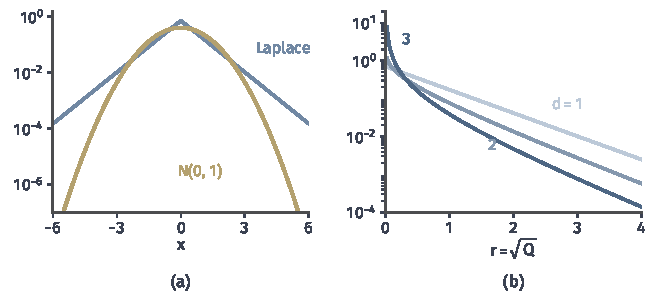
\includegraphics[width=112mm]{figures/07-probability/01-elementary-probability/matplotlib/mvd-laplace-shape/figure.pdf}
  \caption{多元Laplace的形状，$\bm{\mu}=\bm{0}$，$\bm{\Sigma}=\bm{I}_d$，纵轴取对数。(a)一个分量的密度：尺度$b=1/\sqrt2$的Laplace密度（蓝）与方差同为$1$的$\mathcal{N}(0,1)$密度（黄）；Laplace在中心更尖，在远处更厚。(b)沿射线的联合密度随$r=\sqrt Q$的变化，$d=1,2,3$（蓝色由浅到深），由式~\eqref{eq:mvd-laplace-density}数值积分；$d=2,3$时中心处趋于无穷。}
  \label{fig:mvd-laplace-shape}
\end{BookInlineFigure}

\subsection{边缘与共同尺度}
\label{sec:mvd-laplace-marginal}

\paragraph{边缘是一元Laplace}
取出第$i$个分量，$X_i=\mu_i+\sqrt W\,Z_i$，$Z_i\sim\mathcal{N}(0,\Sigma_{i,i})$，$W$不变。这就是$d=1$的构造，由上面的计算，$X_i$服从位置$\mu_i$、尺度
\begin{equation}
 b_i=\sqrt{\Sigma_{i,i}/2}
 \label{eq:mvd-laplace-marginal-scale}
\end{equation}
的一元Laplace分布，尺度的含义与第~\ref{chap:common-distributions}章相同。同理，$\bm{a}^{\top}\bm{X}$服从尺度为$\sqrt{\bm{a}^{\top}\bm{\Sigma}\bm{a}/2}$的一元Laplace分布，任意一组分量服从相应子矩阵的多元Laplace分布。

与同方差的高斯相比，Laplace边缘在中心更尖、远处更厚。图~\ref{fig:mvd-laplace-shape}(a)中两者方差都是$1$：Laplace在$0$处的密度是$1/\sqrt2\approx0.707$，高斯是$0.399$；而$\mathbb{P}(\lvert X_i\rvert>3)$，Laplace为$\mathrm{e}^{-3\sqrt2}\approx0.0144$，高斯约为$0.0027$。

\paragraph{共同尺度造成依赖}
取$\bm{\mu}=\bm{0}$、$\bm{\Sigma}=\bm{I}_2$。两个分量的协方差为$0$，边缘都是尺度$1/\sqrt2$的Laplace分布。它们是否独立？看中心化分量的交叉四阶矩。由$W$、$Z_1$、$Z_2$相互独立，
\[
 \mathbb{E}[X_1^{2}X_2^{2}]=\mathbb{E}[W^{2}]\,\mathbb{E}[Z_1^{2}]\,\mathbb{E}[Z_2^{2}]=2 ,
\]
这里用了$\mathbb{E}[W^{2}]=\Gamma(3)=2$。而$\mathbb{E}[X_1^{2}]\,\mathbb{E}[X_2^{2}]=1$。

若$X_1$与$X_2$独立，则$X_1^{2}$与$X_2^{2}$独立，乘积的期望应等于期望之积。现在$2\neq1$，所以两者不独立，$\operatorname{Cov}(X_1^{2},X_2^{2})=1>0$。与t分布一样，共同尺度$W$同时放大或缩小两个分量的大小，而符号由$Z_1$、$Z_2$独立决定，协方差看不到这种依赖。

\paragraph{与乘积模型对照}
现在另取两个独立的尺度，$Y_i=\sqrt{W_i}\,Z_i$，$W_1,W_2,Z_1,Z_2$相互独立。由一元计算，$Y_1$、$Y_2$也是尺度$1/\sqrt2$的Laplace变量，而且相互独立，联合密度是边缘之积，
\[
 f_{\bm{Y}}(y_1,y_2)=\frac12\exp\bigl(-\sqrt2(\lvert y_1\rvert+\lvert y_2\rvert)\bigr) .
\]
两个模型的边缘相同，均值都是$\bm{0}$，协方差矩阵都是$\bm{I}_2$。

可是它们的联合分布不同。乘积模型的交叉四阶矩是$\mathbb{E}[Y_1^{2}]\,\mathbb{E}[Y_2^{2}]=1$，不是$2$。几何上，椭圆型模型的等密度线是圆，乘积模型的等密度线是菱形$\lvert y_1\rvert+\lvert y_2\rvert=c$，图~\ref{fig:mvd-laplace-contours}。菱形的尖角落在坐标轴上：乘积模型容易出现“一个分量大、另一个分量小”的点；椭圆型模型的大值往往两个分量一起出现。

\begin{BookInlineFigure}
  \centering
  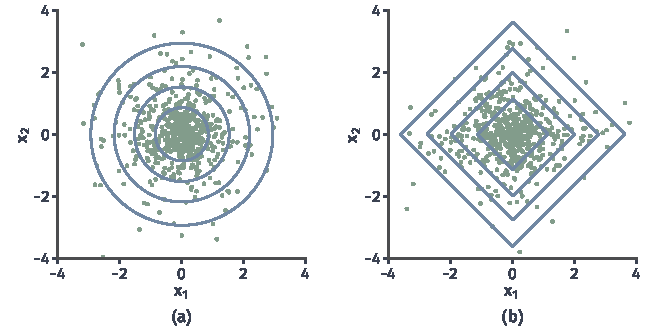
\includegraphics[width=112mm]{figures/07-probability/01-elementary-probability/matplotlib/mvd-laplace-contours/figure.pdf}
  \caption{边缘与协方差都相同的两个模型，各分量都是尺度$1/\sqrt2$的Laplace分布，协方差矩阵为$\bm{I}_2$。(a)椭圆型多元Laplace，等密度线是圆。(b)独立分量的乘积模型，等密度线是菱形。蓝线是密度等于$0.1,0.03,0.01,0.003$的等值线，绿点是各$600$个样本（种子$41$、$42$）。}
  \label{fig:mvd-laplace-contours}
\end{BookInlineFigure}

选哪一个版本，取决于数据的生成方式。各坐标的波动来自同一个源头，比如整个系统的状态忽强忽弱，椭圆型更合适；各坐标各自独立地出现尖峰，乘积模型更合适。两者都可以称为“多元Laplace”，使用时要说明采用的是哪一种构造。
